% Relatório do trabalho final: forma de gotas pendentes como problema de otimização.
%
% Compilar, de dentro de relatorio/:
%   pdflatex relatorio && biber relatorio && pdflatex relatorio && pdflatex relatorio
% As figuras (figuras/) e tabelas (tabelas/) são geradas por gerar_figuras.py.
\documentclass[12pt, oneside, a4paper, english, brazil]{abntex2}

\usepackage[T1]{fontenc}
\usepackage[utf8]{inputenc}
\usepackage{lmodern}
\usepackage{mathpazo}
\usepackage{indentfirst}
\usepackage{microtype}
\usepackage{amsmath, amssymb, amsthm}
\usepackage{graphicx}
\usepackage{booktabs}
\usepackage{float}
\usepackage{algorithm}
\usepackage{algpseudocode}
\usepackage{xcolor}
\usepackage{siunitx}
\usepackage{csquotes}
\usepackage[style=abnt, backend=biber]{biblatex}
\addbibresource{referencias.bib}

% citações com o sobrenome em caixa mista, como no relatório anterior
\AtEveryCite{\let\MakeCapital\relax}

\sisetup{output-decimal-marker = {,}, exponent-product = \cdot,
         group-digits = none, per-mode = symbol}
\graphicspath{{figuras/}}
\hypersetup{colorlinks = true, linkcolor = black, citecolor = black,
            urlcolor = black, filecolor = black,
            pdftitle = {Forma de gotas pendentes como um problema de otimização}}

% ambientes numerados por seção, no formato do relatório anterior ("3.1.1 Definição:")
\newtheoremstyle{relatorio}{\topsep}{\topsep}{\normalfont}{}{\bfseries}{:}{.5em}
  {\thmnumber{#2}\thmname{ #1}\thmnote{ (#3)}}
\newtheoremstyle{relatorioit}{\topsep}{\topsep}{\itshape}{}{\bfseries}{:}{.5em}
  {\thmnumber{#2}\thmname{ #1}\thmnote{ (#3)}}
\newtheoremstyle{problema}{\topsep}{\topsep}{\normalfont}{}{\bfseries}{}{\newline}
  {\thmname{#1}\thmnumber{ #2}\thmnote{ (#3)}}
\theoremstyle{relatorio}
\newtheorem{definicao}{Definição}[section]
\theoremstyle{relatorioit}
\newtheorem{teorema}[definicao]{Teorema}
\newtheorem{proposicao}[definicao]{Proposição}
\theoremstyle{problema}
\newtheorem{problema}{Problema}[section]

% algoritmos em português
\floatname{algorithm}{Algoritmo}
\algrenewcommand\algorithmicrequire{\textbf{Entradas:}}
\algrenewcommand\algorithmicensure{\textbf{Saídas:}}
\algrenewcommand\algorithmicwhile{\textbf{enquanto}}
\algrenewcommand\algorithmicdo{\textbf{faça}}
\algrenewcommand\algorithmicend{\textbf{fim}}

% nomes de arquivos e funções; a linha pode quebrar depois de "_"
\newcommand{\code}[1]{{\renewcommand{\_}{\textunderscore\allowbreak}\texttt{#1}}}
\setlength{\emergencystretch}{2em}
% sumário em uma página, como no relatório anterior
\setlength{\cftbeforechapterskip}{0.5em}
\newcommand{\Vh}{\hat V}
\newcommand{\dhat}{\hat d}
\newcommand{\lh}{\hat\lambda}
\newcommand{\Eh}{\hat E}
\DeclareMathOperator*{\argmin}{arg\,min}

\titulo{Forma de gotas pendentes como um problema de otimização: método do tiro, SLSQP e lagrangiano aumentado}
\autor{Fabio Kauã Araujo da Silva -- 16311045 \\
Gabriel Inumaru Esteves -- 15453487 \\
Kainã Alves Tureso -- 15466391 \\
Matheus Spinelli de Paiva -- 14598682 \\
Pedro Luís Anghievisck -- 15656521}
\local{São Carlos -- SP}
\data{\today}

\begin{document}

\pretextual
\imprimircapa

\textual
\setcounter{page}{1}
\pdfbookmark[0]{\contentsname}{toc}
\tableofcontents
\cleardoublepage

% ---------------------------------------------------------------------------
\chapter{Introdução}

Uma gota pendurada na ponta de uma agulha assume a forma que equilibra a tensão
superficial, que tende a reduzir a área da interface, e a gravidade, que puxa o
líquido para baixo. Essa forma é tão sensível às propriedades do líquido que a sua
medição é a base da tensiometria de gota pendente, uma das técnicas mais usadas para
determinar a tensão superficial: fotografa-se a gota e ajusta-se a tensão
superficial até que o perfil teórico coincida com o observado \parencite{berry2015}.

O perfil teórico é tradicionalmente obtido integrando a equação de Young--Laplace,
escrita como um sistema de equações diferenciais ordinárias (EDO) ao longo do contorno
da gota \parencite{hartland1976}. Existe, porém, uma formulação equivalente que é
natural no contexto deste curso: a forma de equilíbrio é a superfície que minimiza a
energia total, de superfície mais potencial gravitacional, entre todas as superfícies
que encerram um volume dado \parencite{degennes2004}. Trata-se de um problema de
otimização não linear com uma restrição de igualdade, e o multiplicador de Lagrange
associado ao volume tem significado físico: é a diferença de pressão através da
interface.

Neste relatório resolvemos o problema das duas formas. Primeiro integramos a EDO
pelo método de Runge--Kutta de quarta ordem e usamos o método do tiro para impor o
volume. Em seguida discretizamos o perfil e minimizamos a energia com dois métodos: o
SLSQP, um método de programação quadrática sequencial disponível no SciPy
\parencite{kraft1988, virtanen2020}, e o método do lagrangiano aumentado, que
implementamos a partir do Algoritmo 5.2 de \textcite{martins2021}. As soluções da EDO
servem de referência para validar a otimização, inclusive o multiplicador de
Lagrange. Por fim, aplicamos a formulação variacional a uma gota tridimensional
pendurada em um bico quadrado, caso em que a EDO axissimétrica deixa de valer.

% ---------------------------------------------------------------------------
\chapter{Objetivos}

O objetivo deste trabalho é determinar a forma de equilíbrio de gotas pendentes
formulando-a como um problema de otimização com restrição e comparar métodos para
resolvê-lo. Mais especificamente, buscamos:

\begin{itemize}
  \item obter, pelo método do tiro, perfis de referência de gotas pendentes de água
    em um bico de raio \qty{1}{mm}, até a gota de volume máximo;
  \item formular a minimização da energia com volume fixo e resolvê-la com o SLSQP e
    com o método do lagrangiano aumentado;
  \item verificar se os métodos de otimização reproduzem a forma e a pressão obtidas
    pela EDO e estudar a convergência com o refinamento da discretização;
  \item avaliar o custo computacional e o comportamento do lagrangiano aumentado,
    inclusive perto do volume máximo;
  \item aplicar a formulação a uma gota tridimensional pendurada em um bico quadrado.
\end{itemize}

% ---------------------------------------------------------------------------
\chapter{Revisão Bibliográfica}

\section{Capilaridade e a equação de Young--Laplace}

\begin{definicao}
A tensão superficial $\gamma$ de uma interface é a energia necessária para aumentar
sua área em uma unidade \parencite{degennes2004}. Para a interface entre água e ar a
\qty{20}{\celsius}, $\gamma \approx \qty{0.0728}{N/m}$.
\end{definicao}

Como uma interface curva tende a diminuir de área, ela só fica em equilíbrio se houver
uma diferença de pressão $\Delta p$ entre os seus dois lados. Essa diferença é dada pela
equação de Young--Laplace \parencite{degennes2004}:
\begin{equation}
  \Delta p = \gamma \left( \frac{1}{R_1} + \frac{1}{R_2} \right) = \gamma\,\kappa,
  \label{eq:young-laplace}
\end{equation}
em que $R_1$ e $R_2$ são os raios de curvatura principais da superfície e $\kappa$ é a
soma das curvaturas principais. Em uma gota em repouso sob a gravidade, a pressão no
líquido é hidrostática. Medindo $z$ para cima a partir do ápice, que é o ponto mais
baixo da gota pendente, e chamando de $\Delta p_0$ a diferença de pressão no ápice,
\begin{equation}
  \Delta p(z) = \Delta p_0 - \Delta\rho\, g\, z,
  \label{eq:hidrostatica}
\end{equation}
em que $\Delta\rho$ é a diferença de densidade entre o líquido e o ar.

Tomando como escala de comprimento o raio $a$ do bico, escrevemos $\hat r = r/a$,
$\hat z = z/a$, $\hat s = s/a$ e $\Vh = V/a^3$, e definimos os parâmetros adimensionais
\begin{equation}
  A = \frac{a\, \Delta p_0}{\gamma}, \qquad B = \frac{\Delta\rho\, g\, a^2}{\gamma}.
  \label{eq:adimensionais}
\end{equation}
$A$ é a pressão adimensional no ápice, e $B$, o número de Bond, mede a importância da
gravidade frente à tensão superficial. Daqui em diante omitimos o acento circunflexo
das coordenadas quando não houver ambiguidade.

\subsection{Perfil axissimétrico}

Em uma gota axissimétrica, o perfil é uma curva $(r(s), z(s))$ parametrizada pelo
comprimento de arco $s$ a partir do ápice. Chamando de $\theta(s)$ o ângulo entre a
tangente e a horizontal, as duas curvaturas principais são $\mathrm{d}\theta/\mathrm{d}s$
e $\sin\theta/r$, e as equações \eqref{eq:young-laplace} e \eqref{eq:hidrostatica}
tornam-se o sistema \parencite{hartland1976}
\begin{equation}
  \frac{\mathrm{d}r}{\mathrm{d}s} = \cos\theta, \quad
  \frac{\mathrm{d}z}{\mathrm{d}s} = \sin\theta, \quad
  \frac{\mathrm{d}\theta}{\mathrm{d}s} = A - B z - \frac{\sin\theta}{r}, \quad
  \frac{\mathrm{d}V}{\mathrm{d}s} = \pi r^2 \sin\theta, \quad
  \frac{\mathrm{d}S}{\mathrm{d}s} = 2\pi r,
  \label{eq:edo}
\end{equation}
em que $V$ e $S$ são o volume e a área acumulados desde o ápice. No ápice, o termo
$\sin\theta/r$ é indeterminado; por isso a integração começa em um $s = \varepsilon$
pequeno, com os valores da série de Taylor da solução:
\begin{equation}
  r \approx \varepsilon - \frac{A^2 \varepsilon^3}{24}, \quad
  z \approx \frac{A \varepsilon^2}{4}, \quad
  \theta \approx \frac{A \varepsilon}{2} - \frac{A B \varepsilon^3}{16}, \quad
  V \approx \frac{\pi A \varepsilon^4}{8}, \quad
  S \approx \pi \varepsilon^2.
  \label{eq:taylor}
\end{equation}

Para cada valor de $A$, a integração produz um perfil. A gota pendente é o trecho entre
o ápice e um ponto em que $r = 1$, isto é, em que o perfil alcança a borda do bico. Como
o perfil pode cruzar $r = 1$ mais de uma vez, um mesmo valor de $A$ pode corresponder a
várias gotas, com volumes e alturas diferentes.

\subsection{Volume máximo}

O volume de uma gota pendente não pode crescer indefinidamente: existe um volume
máximo $\Vh^*$ acima do qual não há equilíbrio, e a gota se desprende do bico
\parencite{padday1973}. Na família de soluções de \eqref{eq:edo}, $\Vh^*$ aparece como
o máximo do volume em função de $A$.

\section{Formulação variacional}

A energia de uma gota com volume fixo é a soma da energia de superfície com a energia
potencial gravitacional:
\begin{equation}
  E = \gamma\, \mathrm{\acute{A}rea}(S) + \int_\Omega \Delta\rho\, g\, z \,\mathrm{d}V,
  \label{eq:energia}
\end{equation}
em que $S$ é a superfície livre e $\Omega$ é o líquido. Nesta formulação medimos $z$ a
partir do plano do bico, positivo para cima, de modo que a gota fica em $z < 0$. Pelo
teorema da divergência,
$\int_\Omega z \,\mathrm{d}V = \oint_{\partial\Omega} \tfrac{z^2}{2}\, n_z \,\mathrm{d}A$ e
$V = \tfrac{1}{3}\oint_{\partial\Omega} \mathbf{x}\cdot\mathbf{n} \,\mathrm{d}A$. A
fronteira $\partial\Omega$ é formada pela superfície livre e pelo disco do bico, que
está no plano $z = 0$, onde $z^2$ e $\mathbf{x}\cdot\mathbf{n} = z$ se anulam. Por isso
as duas integrais podem ser calculadas só sobre a superfície livre. Em forma
adimensional,
\begin{equation}
  \Eh = \frac{E}{\gamma a^2} = \hat{\mathcal A} + \frac{B}{2}\int_S \hat z^2\, n_z \,\mathrm{d}\hat{\mathcal A},
  \qquad
  \Vh = \frac{1}{3}\int_S \hat{\mathbf{x}}\cdot\mathbf{n} \,\mathrm{d}\hat{\mathcal A}.
  \label{eq:energia-adim}
\end{equation}

\begin{problema}
Dado $\Vh_0 > 0$, minimizar $\Eh(S)$ entre as superfícies $S$ cuja borda está presa à
borda do bico, sujeito a $\Vh(S) = \Vh_0$.
\label{prob:continuo}
\end{problema}

A condição de primeira ordem desse problema recupera a equação de Young--Laplace. Para
um deslocamento normal $\delta n$ da superfície, a primeira variação da área é
$\int_S \hat\kappa\, \delta n \,\mathrm{d}\hat{\mathcal A}$, a da energia potencial é
$\int_S B \hat z\, \delta n \,\mathrm{d}\hat{\mathcal A}$ e a do volume é
$\int_S \delta n \,\mathrm{d}\hat{\mathcal A}$. Pela regra dos multiplicadores de
Lagrange, existe $\lh$ tal que $\delta \Eh = \lh\, \delta \Vh$ para todo $\delta n$, ou
seja,
\begin{equation}
  \hat\kappa + B \hat z = \lh \quad \text{em toda a superfície livre.}
  \label{eq:euler-lagrange}
\end{equation}
Comparando com \eqref{eq:young-laplace} e \eqref{eq:hidrostatica}, $\lh$ é a diferença
de pressão adimensional no plano do bico. No ápice, $\hat z = -\dhat$ e
$\hat\kappa = A$, o que leva ao resultado abaixo.

\begin{proposicao}
O multiplicador de Lagrange da restrição de volume do Problema~\ref{prob:continuo} é
$\lh = A - B\dhat$, em que $\dhat$ é a altura da gota, isto é, a distância do ápice ao plano
do bico.
\label{prop:multiplicador}
\end{proposicao}

\section{Otimização com restrições}

Os métodos usados neste trabalho resolvem problemas da forma geral abaixo.

\begin{problema}
\begin{equation}
  \min_{x \in \mathbb{R}^n} \; f(x) \quad \text{sujeito a} \quad
  h(x) = 0, \quad g(x) \le 0,
  \label{eq:problema-geral}
\end{equation}
com $h\colon \mathbb{R}^n \to \mathbb{R}^{m_h}$ e $g\colon \mathbb{R}^n \to \mathbb{R}^{m_g}$.
\label{prob:geral}
\end{problema}

\begin{definicao}
O lagrangiano do Problema~\ref{prob:geral} é
$\mathcal{L}(x, \lambda, \sigma) = f(x) + \lambda^{\mathsf T} h(x) + \sigma^{\mathsf T} g(x)$,
em que $\lambda \in \mathbb{R}^{m_h}$ e $\sigma \in \mathbb{R}^{m_g}$ são os multiplicadores
de Lagrange \parencite{martins2021}.
\end{definicao}

\begin{teorema}[condições de Karush--Kuhn--Tucker]
Seja $x^*$ um minimizador local do Problema~\ref{prob:geral} em que os gradientes das
restrições ativas são linearmente independentes. Então existem $\lambda^*$ e $\sigma^*$
tais que $\nabla f(x^*) + J_h(x^*)^{\mathsf T} \lambda^* + J_g(x^*)^{\mathsf T}\sigma^* = 0$,
$h(x^*) = 0$, $g(x^*) \le 0$, $\sigma^* \ge 0$ e $\sigma_j^*\, g_j(x^*) = 0$ para todo
$j$ \parencite[cap.~12]{nocedal2006}.
\end{teorema}

\subsection{Programação quadrática sequencial}

Os métodos de programação quadrática sequencial (SQP) resolvem, a cada iteração, um
subproblema formado por um modelo quadrático do lagrangiano e pela linearização das
restrições, e atualizam uma aproximação da hessiana por fórmulas quasi-Newton
\parencite{nocedal2006, martins2021}. O SLSQP \parencite{kraft1988}, usado aqui por meio
de \code{scipy.optimize.minimize}, é uma implementação desse tipo em que o subproblema
é resolvido como um problema de mínimos quadrados. Quando as derivadas não são
fornecidas, o SciPy as estima por diferenças finitas.

\subsection{Penalidade quadrática}

Os métodos de penalidade trocam o problema com restrições por uma sequência de
problemas sem restrições \parencite[seção~5.4]{martins2021}. Na penalidade quadrática,
minimiza-se
\begin{equation}
  \hat f(x; \mu) = f(x) + \frac{\mu}{2} \sum_{j} h_j(x)^2
  \label{eq:penalidade}
\end{equation}
para valores crescentes do parâmetro de penalidade $\mu$. Comparando as condições de
otimalidade de $\hat f$ e do lagrangiano, conclui-se que, no minimizador de $\hat f$,
$h_j \approx \lambda_j^*/\mu$. A viabilidade, portanto, só é alcançada no limite
$\mu \to \infty$, e o condicionamento da hessiana de $\hat f$, que piora com $\mu$,
torna os subproblemas cada vez mais difíceis.

\subsection{Lagrangiano aumentado}
\label{sec:la}

O método do lagrangiano aumentado \parencite{hestenes1969, powell1969} contorna esse
dilema somando a penalidade ao lagrangiano, e não à função objetivo:
\begin{equation}
  \hat f(x; \lambda, \mu) = f(x) + \sum_j \lambda_j h_j(x) + \frac{\mu}{2} \sum_j h_j(x)^2.
  \label{eq:lagrangiano-aumentado}
\end{equation}
A condição de otimalidade de \eqref{eq:lagrangiano-aumentado},
$\nabla f + \sum_j (\lambda_j + \mu h_j) \nabla h_j = 0$, comparada com a do lagrangiano,
$\nabla f + \sum_j \lambda^*_j \nabla h_j = 0$, sugere a estimativa
$\lambda_j^* \approx \lambda_j + \mu h_j(x)$ e a atualização
\begin{equation}
  \lambda \leftarrow \lambda + \mu\, h(x).
  \label{eq:atualizacao}
\end{equation}
Daí vem $h_j \approx (\lambda_j^* - \lambda_j)/\mu$: à medida que a estimativa do
multiplicador melhora, a violação diminui sem que $\mu$ precise crescer
indefinidamente \parencite{martins2021}. O método completo está no
Algoritmo~\ref{alg:lagrangiano-aumentado}.

\begin{algorithm}[H]
\caption{Método do lagrangiano aumentado \parencite[Alg.~5.2]{martins2021}}
\label{alg:lagrangiano-aumentado}
\begin{algorithmic}[1]
  \Require ponto inicial $x_0$; multiplicadores $\lambda_0 = 0$; penalidade inicial
    $\mu_0 > 0$; fator de aumento $\rho > 1$
  \Ensure ponto ótimo $x^*$ e o valor $f(x^*)$
  \State $k \gets 0$
  \While{não convergiu}
    \State $x_k^* \gets \argmin_x \hat f(x; \lambda_k, \mu_k)$, partindo de $x_k$
    \State $\lambda_{k+1} \gets \lambda_k + \mu_k\, h(x_k^*)$ \Comment{atualiza os multiplicadores}
    \State $\mu_{k+1} \gets \rho\, \mu_k$ \Comment{aumenta a penalidade}
    \State $x_{k+1} \gets x_k^*$ \Comment{novo ponto de partida}
    \State $k \gets k + 1$
  \EndWhile
\end{algorithmic}
\end{algorithm}

Restrições de desigualdade podem ser incluídas trocando, em
\eqref{eq:lagrangiano-aumentado}, cada $h_j$ por
$\bar g_j(x) = \max\left(g_j(x), -\sigma_j/\mu\right)$ e atualizando
$\sigma \gets \sigma + \mu \bar g(x) = \max\left(0, \sigma + \mu g(x)\right)$
\parencite{rockafellar1973, martins2021}.

Os subproblemas do Algoritmo~\ref{alg:lagrangiano-aumentado} não têm restrições, a
menos de limites simples nas variáveis. Para eles usamos o L-BFGS-B
\parencite{byrd1995}, um método quasi-Newton de memória limitada que trata limites
inferiores e superiores diretamente, por projeção.

\section{Métodos numéricos auxiliares}

Para integrar \eqref{eq:edo} usamos o método de Runge--Kutta de quarta ordem (RK4) com
passo fixo e, para ajustar $A$, o método da secante \parencite{burden2008}. As
integrais da formulação variacional são calculadas por quadratura: em cada segmento
do perfil bidimensional, pela regra de Gauss--Legendre de três pontos, exata para
polinômios de grau até 5 \parencite{burden2008}; em cada triângulo da malha
tridimensional, pelas regras de \textcite{strang1973}, tabeladas por
\textcite{burkardt}.

% ---------------------------------------------------------------------------
\chapter{Procedimentos e Métodos}

\section{Modelagem Matemática}

Todas as contas usam água a \qty{20}{\celsius} em um bico de raio
$a = \qty{1}{mm}$: $\gamma = \qty{0.0728}{N/m}$, $\Delta\rho = \qty{1000}{kg/m^3}$ e
$g = \qty{9.81}{m/s^2}$, o que dá $B = \num{0.134753}$.

Na versão axissimétrica, o perfil é aproximado por uma poligonal de $N$ pontos
$P_i = (r_i, z_i)$, do ponto $P_0 = (1, 0)$, na borda do bico, até $P_{N-1}$, no eixo. O
ponto de partida é a calota esférica de volume $\Vh_0$ que passa pela borda do bico,
cujo centro $c = (0, -h)$ é obtido pelo método de Newton. Cada ponto se move sobre a
reta que o liga ao centro da calota:
\begin{equation}
  P_i(x) = P_i^0 + x_i \left(P_i^0 - c\right), \qquad i = 0, \ldots, N - 1.
  \label{eq:parametrizacao}
\end{equation}
O ponto da borda do bico fica fixo ($x_0 = 0$), e os limites $x_i > -1$ impedem que um
ponto atravesse o centro. Cada segmento do perfil gera, ao girar em torno do eixo, um
tronco de cone, e as integrais \eqref{eq:energia-adim} sobre ele são polinômios das
coordenadas dos extremos. Sendo $(r_1, z_1)$ e $(r_2, z_2)$ os extremos de um segmento
e $\ell$ o seu comprimento, as contribuições do segmento são
\begin{align}
  \frac{\Eh_{\mathrm{seg}}}{\pi} &= \ell\,(r_1 + r_2) + \frac{B}{12}(r_2 - r_1)
    \left[ r_1 \left(3z_1^2 + 2z_1z_2 + z_2^2\right) + r_2 \left(z_1^2 + 2z_1z_2 + 3z_2^2\right) \right],
  \label{eq:energia-segmento} \\
  \Vh_{\mathrm{seg}} &= \frac{2\pi}{3} \left[ \frac{(z_1 - z_2)\left(r_1^2 + r_1 r_2 + r_2^2\right)}{3}
    + \frac{(r_2 - r_1)\left(2r_1z_1 + r_1z_2 + r_2z_1 + 2r_2z_2\right)}{6} \right].
  \label{eq:volume-segmento}
\end{align}
O código original calcula essas integrais pela regra de Gauss--Legendre de três pontos,
que é exata para esses integrandos; as fórmulas fechadas dão o mesmo valor, a menos de
erros de arredondamento, e permitem calcular o gradiente exato.

\begin{problema}
\begin{equation}
  \min_{x \in \mathbb{R}^N} \; \frac{\Eh(x)}{\pi} \quad \text{sujeito a} \quad
  \Vh(x) = \Vh_0, \quad x_0 = 0, \quad x_i \ge -1 + 10^{-8}, \; i = 1, \ldots, N - 1.
  \label{eq:problema-discreto}
\end{equation}
\label{prob:discreto}
\end{problema}

Como a energia está dividida por $\pi$, o multiplicador do Problema~\ref{prob:discreto},
na convenção $\nabla(\Eh/\pi) = \lh\, \nabla\Vh$, é $\lh = (A - B\dhat)/\pi$ pela
Proposição~\ref{prop:multiplicador}. É com essa normalização que comparamos os
métodos.

\section{Método do tiro}

Para um valor de $A$, integramos \eqref{eq:edo} com o RK4, passo $\Delta s = 0{,}001$,
até $s = 5\pi$, e procuramos os passos em que $r$ cruza o valor 1. Cada cruzamento,
refinado por interpolação linear entre os dois passos vizinhos, define uma gota com
altura $\dhat$ e volume $\Vh(A)$. O método do tiro ajusta $A$ pelo método da secante até
que $\Vh(A) = \Vh_0$, com tolerância $10^{-10}$. Os intervalos iniciais da secante
dependem do volume e são os mesmos usados em \code{run/comparison.py}.

\section{Implementação Computacional}

O código foi escrito em Python, com NumPy \parencite{harris2020}, SciPy
\parencite{virtanen2020} e Matplotlib \parencite{hunter2007}. Os resultados deste
relatório foram obtidos com Python 3.14.5, NumPy 2.4.6, SciPy 1.18.0 e
Matplotlib 3.11.0. A implementação do método do lagrangiano aumentado, os testes
automatizados e a redação inicial deste relatório contaram com o auxílio do assistente
Claude \parencite{claude2026}. O repositório está organizado da seguinte forma:

\begin{itemize}
  \item \code{src/2D}: integração da EDO (\code{solve\_PVI.py} e \code{droplet.py}),
    otimização com SLSQP (\code{droplet\_optimization.py}), método do lagrangiano
    aumentado (\code{augmented\_lagrangian.py}), geometria e quadratura
    (\code{objects.py} e \code{quadrature.py});
  \item \code{src/3D}: malha triangular (\code{mesh.py}), quadratura em triângulos
    (\code{quadrature\_triangle.py}) e otimização (\code{optimization\_3d.py});
  \item \code{run}: roteiros de experimentos (\code{pendant.py}, \code{sessile.py} e
    \code{comparison.py});
  \item \code{tests}: testes automatizados, executados com o \code{pytest};
  \item \code{relatorio}: este relatório e o roteiro \code{gerar\_figuras.py}, que
    produz todas as figuras e tabelas a partir do código.
\end{itemize}

\subsection{Estratégias de Resolução}

Foram usadas quatro abordagens:

\begin{itemize}
  \item \textbf{EDO e método do tiro} (\code{droplet.py}): fornece as soluções de
    referência, como descrito na seção anterior.
  \item \textbf{SLSQP} (\code{find\_droplet\_optimization}): resolve o
    Problema~\ref{prob:discreto} com \code{scipy.\allowbreak optimize.\allowbreak minimize} (método
    \code{SLSQP}, \code{ftol} $= 10^{-12}$), com gradientes estimados por diferenças
    finitas. O multiplicador é estimado ao final por mínimos quadrados, a partir de
    $\nabla\Eh$ e $\nabla\Vh$.
  \item \textbf{Lagrangiano aumentado} (\code{find\_droplet\_augmented\_lagrangian}):
    aplica o Algoritmo~\ref{alg:lagrangiano-aumentado} ao Problema~\ref{prob:discreto}.
    Seguindo a recomendação de \textcite[Dica 5.3]{martins2021} de normalizar as
    restrições, usamos $h(x) = \Vh(x)/\Vh_0 - 1$. Os subproblemas são resolvidos pelo
    L-BFGS-B com o gradiente exato de \eqref{eq:energia-segmento} e
    \eqref{eq:volume-segmento}, e os limites $x_i \ge -1 + 10^{-8}$ ficam a cargo do
    próprio L-BFGS-B. Usamos $\mu_0 = 1000$, $\rho = 2$ e o critério de parada
    $|h(x)| \le 10^{-10}$. O multiplicador sai diretamente do método: como o
    lagrangiano é $\Eh/\pi + \lambda\,(\Vh/\Vh_0 - 1)$, temos $\lh = -\lambda/\Vh_0$.
    Acrescentamos duas salvaguardas que não fazem parte do algoritmo do livro: um teto
    $\mu \le 10^{12}$ e uma parada por estagnação, discutida na
    Seção~\ref{sec:discussao}.
  \item \textbf{Gota tridimensional} (\code{find\_droplet\_optimization\_3d}): a
    superfície é uma malha de triângulos formada por uma calota (hemisfério de raio 1
    com centro em $z = -0{,}2$) e por um ``colar'' de triângulos que a liga ao contorno
    do bico, um quadrado $[-1, 1]^2$ no plano $z = 0$. As variáveis são, como em
    \eqref{eq:parametrizacao}, os deslocamentos radiais dos vértices da calota; os
    vértices do bico ficam fixos. As integrais \eqref{eq:energia-adim} são calculadas
    com a regra de Strang--Fix de quatro pontos, exata até grau 3, e o problema é
    resolvido pelo SLSQP com diferenças finitas. A opção \code{fix\_boundary} fixa
    também o anel em que a calota foi cortada.
\end{itemize}

\subsection{Roteiro de Execução}

Para reproduzir os resultados, a partir da raiz do repositório:

\begin{enumerate}
  \item \textbf{Testes} (\code{python -m pytest tests -q}): conferem as correções do
    código e o lagrangiano aumentado, inclusive o Exemplo 5.8 de \textcite{martins2021}.
  \item \textbf{Comparação rápida} (\code{python augmented\_lagrangian.py}, de dentro
    de \code{src/2D}): compara a EDO, o SLSQP e o lagrangiano aumentado para
    $\Vh = \Vh^*/3$.
  \item \textbf{Experimentos} (\code{python pendant.py}, \code{sessile.py} ou
    \code{comparison.py}, de dentro de \code{run}): o tipo de gráfico é escolhido pela
    variável no início de cada arquivo.
  \item \textbf{Figuras e tabelas} (\code{python gerar\_figuras.py}, de dentro de
    \code{relatorio}): usa os resultados guardados em \code{relatorio/dados}; a opção
    \code{--recalcular} refaz todas as contas.
  \item \textbf{Relatório}: \code{pdflatex}, \code{biber} e mais duas vezes
    \code{pdflatex} sobre \code{relatorio.tex}.
\end{enumerate}

% ---------------------------------------------------------------------------
\chapter{Resultados}

\section{Análise e Desempenho}

Todas as figuras e tabelas deste capítulo foram geradas por
\code{relatorio/gerar\_figuras.py}, que executa o código do repositório; o conjunto
completo de contas leva cerca de quatro minutos.

\subsection{Gotas de referência pelo método do tiro}

A Figura~\ref{fig:familia} mostra perfis obtidos pelo método do tiro para volumes
entre $\Vh = 1$ e o volume máximo. As gotas pequenas são quase esféricas, porque a
tensão superficial domina; à medida que o volume cresce, a gravidade alonga a gota, que
passa a ter um pescoço logo abaixo do bico. A altura vai de $\dhat = \num{0.576}$, para
$\Vh = 1$, até $\dhat = \num{5.371}$, para $\Vh^*$.

\begin{figure}[H]
  \centering
  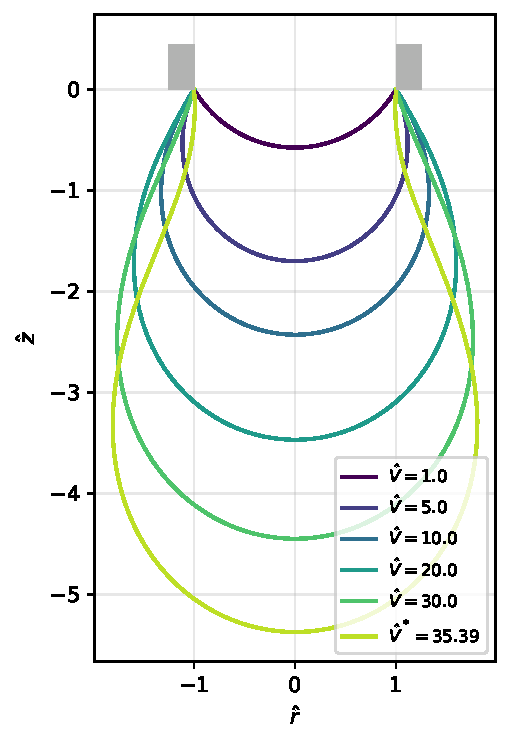
\includegraphics[width=0.5\textwidth]{familia_tiro.pdf}
  \caption{Perfis de gotas pendentes obtidos pelo método do tiro; o bico, em cinza,
    está em $\hat z = 0$ (Autoria própria)}
  \label{fig:familia}
\end{figure}

A Figura~\ref{fig:curva-VA} mostra o volume de todas as gotas encontradas para 219
valores de $A$ entre \num{0.02} e \num{2.2}; cada marcador corresponde a um cruzamento
do perfil com $\hat r = 1$. Dois pontos se destacam:

\begin{itemize}
  \item \textbf{Pressão máxima no ápice}: $A_{\max} = \num{2.0461446}$, com
    $\Vh = \num{2.1722}$. Nesse ponto as duas primeiras interseções se fundem; para
    $A > A_{\max}$ só restam gotas com $\Vh > 5$, vindas de cruzamentos posteriores do
    perfil.
  \item \textbf{Volume máximo}: $\Vh^* = \num{35.394862}$, alcançado em
    $A^* = \num{1.1972112}$ na terceira interseção. Para $A = A^* \pm 10^{-4}$, os
    maiores volumes são \num{35.394707} e \num{35.394648}, ambos menores que $\Vh^*$.
    Em unidades físicas, $\Vh^*$ corresponde a cerca de \qty{35.4}{\micro\liter} de
    água em um bico de raio \qty{1}{mm}.
\end{itemize}

Os dois pontos coincidem com os valores anotados em \code{run/pendant.py}.

\begin{figure}[H]
  \centering
  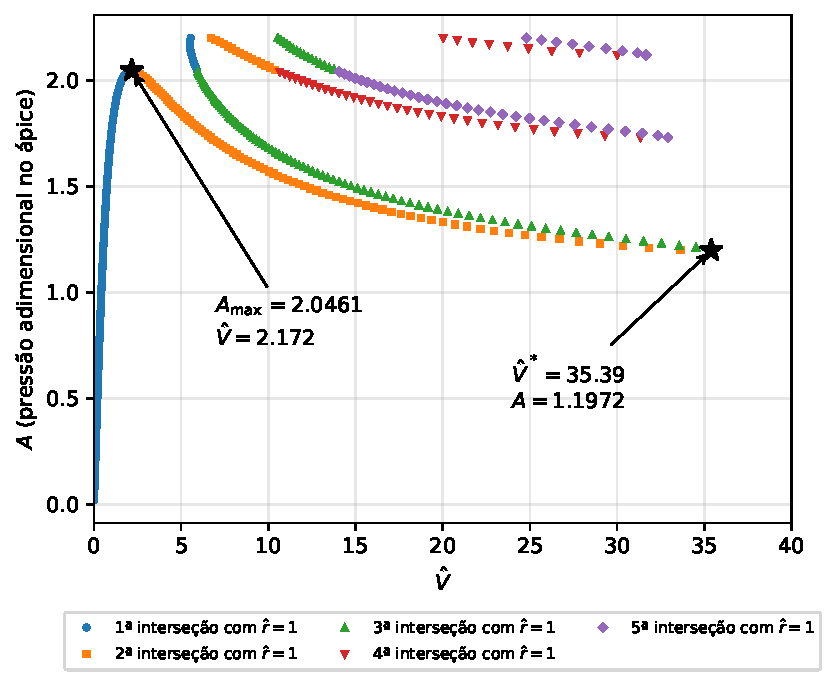
\includegraphics[width=0.8\textwidth]{curva_VA.pdf}
  \caption{Volume das gotas pendentes em função da pressão adimensional no ápice $A$;
    cada marcador indica um cruzamento do perfil com a borda do bico (Autoria própria)}
  \label{fig:curva-VA}
\end{figure}

\subsection{Validação do lagrangiano aumentado}

Antes de aplicar o método à gota, conferimos a implementação no Exemplo 5.8 de
\textcite{martins2021}: minimizar $x_1 + 2x_2$ sujeito a $x_1^2/4 + x_2^2 - 1 = 0$,
com $\mu_0 = \num{0.5}$ e $\rho = \num{1.1}$, partindo de $x_0 = (0, 0)$. A solução
exata é $x^* = (-\sqrt 2, -1/\sqrt 2)$, com multiplicador $\lambda^* = \sqrt 2$. A
Tabela~\ref{tab:exemplo} compara os valores de $\mu_k$ e $\lambda_k$ mostrados na
Figura 5.32 do livro com os nossos, que coincidem em todas as casas decimais
publicadas. O método termina em 20 iterações externas com $\lambda = \num{1.41421357}$,
um erro de \num{7.3e-9}.

\begin{table}[H]
  \centering
  \caption{Exemplo 5.8 de \textcite{martins2021}: penalidade $\mu_k$ e multiplicador
    $\lambda_k$ usados no subproblema $k$ (Autoria própria)}
  \label{tab:exemplo}
  \begin{tabular}{rcccc}
\toprule
 & \multicolumn{2}{c}{Livro (Fig. 5.32)} & \multicolumn{2}{c}{Este trabalho} \\
\cmidrule(lr){2-3}\cmidrule(lr){4-5}
$k$ & $\mu_k$ & $\lambda_k$ & $\mu_k$ & $\lambda_k$ \\
\midrule
0 & \num{0.50} & \num{0.000} & \num{0.5000} & \num{0.000000} \\
2 & \num{0.61} & \num{1.146} & \num{0.6050} & \num{1.145865} \\
9 & \num{1.18} & \num{1.413} & \num{1.1790} & \num{1.413111} \\
\midrule
20 (final) & --- & $\sqrt 2 \approx \num{1.414214}$ & --- & \num{1.414214} \\
\bottomrule
\end{tabular}

\end{table}

\subsection{Comparação dos métodos}

A Tabela~\ref{tab:comparacao} e a Figura~\ref{fig:comparacao} comparam, para três
volumes, a solução da EDO com as soluções do Problema~\ref{prob:discreto} obtidas pelo
SLSQP e pelo lagrangiano aumentado, ambos com $N = 30$ pontos. Os dois métodos de
otimização chegam à mesma solução discreta: para $\Vh^*/3$ e $2\Vh^*/3$, as alturas
diferem em menos de \num{1.4e-6} e os multiplicadores em menos de \num{8.2e-8}. A
diferença para a EDO é o erro da discretização: \qty{0.23}{\percent} na altura para
$\Vh^*/3$ e $2\Vh^*/3$, e \qty{2.2}{\percent} para $\Vh^*$. O lagrangiano aumentado
precisou de 4 ou 5 iterações externas e foi cerca de duas vezes mais rápido que o
SLSQP.

\begin{table}[H]
  \centering
  \caption{Altura $\dhat$ e multiplicador $\lh$ obtidos pelos três métodos, com
    $N = 30$ pontos nos métodos de otimização; para o lagrangiano aumentado, as
    iterações são as externas e, entre parênteses, as do L-BFGS-B (Autoria própria)}
  \label{tab:comparacao}
  \begin{tabular}{llcccc}
\toprule
$\hat V$ & Método & $\hat d$ & $\hat\lambda$ & Iterações & Tempo (s) \\
\midrule
$\hat V^*/3$ & EDO (tiro) & \num{2.638192} & \num{0.367023} & --- & --- \\
 & SLSQP & \num{2.644205} & \num{0.367151} & 33 & \num{0.33} \\
 & Lagr. aumentado & \num{2.644204} & \num{0.367151} & 4 (287) & \num{0.19} \\
\midrule
$2\hat V^*/3$ & EDO (tiro) & \num{3.808177} & \num{0.244863} & --- & --- \\
 & SLSQP & \num{3.817061} & \num{0.245067} & 35 & \num{0.36} \\
 & Lagr. aumentado & \num{3.817059} & \num{0.245067} & 4 (270) & \num{0.19} \\
\midrule
$\hat V^*$ & EDO (tiro) & \num{5.371101} & \num{0.150701} & --- & --- \\
 & SLSQP & \num{5.253629} & \num{0.155718} & 52 & \num{0.49} \\
 & Lagr. aumentado & \num{5.253608} & \num{0.155719} & 5 (361) & \num{0.22} \\
\bottomrule
\end{tabular}

\end{table}

\begin{figure}[H]
  \centering
  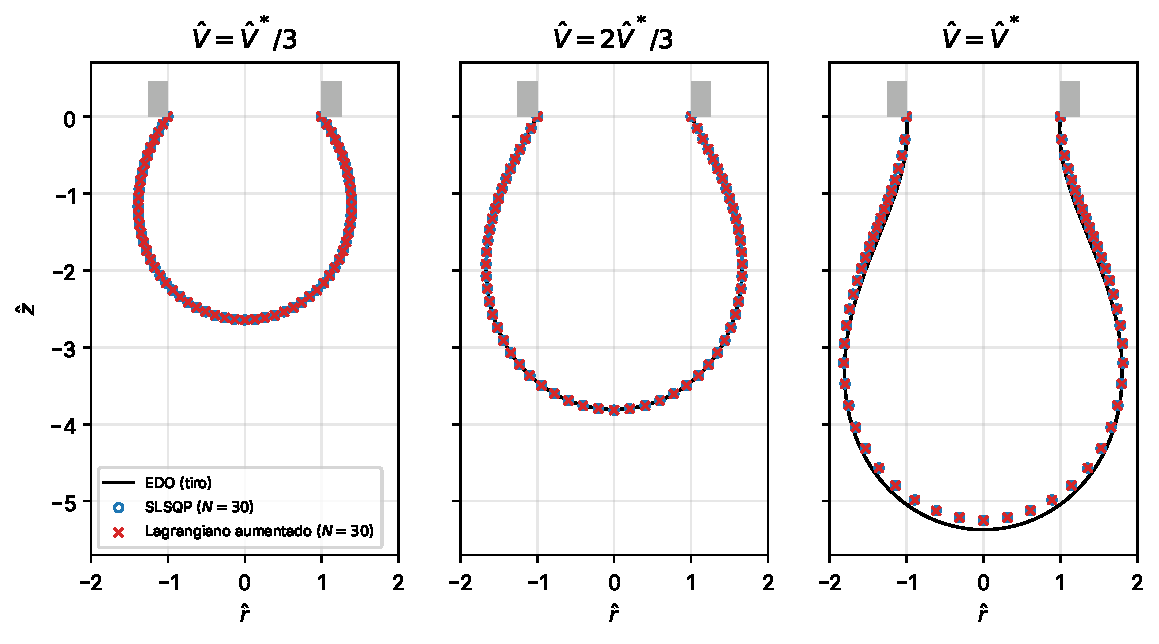
\includegraphics[width=\textwidth]{comparacao_perfis.pdf}
  \caption{Perfis obtidos pela EDO (linha) e pelos dois métodos de otimização com
    $N = 30$ pontos (marcadores) (Autoria própria)}
  \label{fig:comparacao}
\end{figure}

\subsection{Convergência e custo}

Para medir o erro da discretização, resolvemos o caso $\Vh = 2\Vh^*/3$ com
$N = 8$, 16, 32, 64 e 128 pontos (Tabela~\ref{tab:convergencia} e
Figura~\ref{fig:convergencia}). Ao dobrar $N$, o erro no multiplicador cai cerca de
quatro vezes (ordem observada entre \num{2.0} e \num{2.2}) e o erro na altura cai entre
\num{3.4} e \num{3.8} vezes (ordem entre \num{1.8} e \num{1.9}), o que é compatível com
o erro de segunda ordem esperado ao aproximar uma curva suave por uma poligonal. Os
dois métodos têm o mesmo erro, porque resolvem o mesmo problema discreto; a pequena
diferença em $N = 128$ vem da precisão com que cada um resolve o problema.

O tempo, porém, cresce de forma muito diferente. O SLSQP estima os gradientes por
diferenças finitas, o que custa cerca de $N$ avaliações da energia e do volume a cada
iteração, e resolve um subproblema quadrático denso; seu tempo passa de
\qty{0.04}{s}, com $N = 8$, para \qty{5.72}{s}, com $N = 128$. O lagrangiano aumentado
usa o gradiente exato e precisou de 4 a 6 iterações externas em todos os casos; seu
tempo passa de \qty{0.08}{s} para \qty{0.79}{s}, cerca de sete vezes menos que o
SLSQP em $N = 128$.

\begin{table}[H]
  \centering
  \caption{Erro em relação à EDO e tempo de execução para $\Vh = 2\Vh^*/3$; L.A.
    indica o lagrangiano aumentado (Autoria própria)}
  \label{tab:convergencia}
  \begin{tabular}{rcccccc}
\toprule
 & \multicolumn{2}{c}{$|\hat d - \hat d_{EDO}|$} & \multicolumn{2}{c}{$|\hat\lambda - \hat\lambda_{EDO}|$} & \multicolumn{2}{c}{Tempo (s)} \\
\cmidrule(lr){2-3}\cmidrule(lr){4-5}\cmidrule(lr){6-7}
$N$ & SLSQP & L.A. & SLSQP & L.A. & SLSQP & L.A. \\
\midrule
8 & \num{1.08e-01} & \num{1.08e-01} & \num{3.03e-03} & \num{3.03e-03} & \num{0.04} & \num{0.09} \\
16 & \num{2.83e-02} & \num{2.83e-02} & \num{7.39e-04} & \num{7.39e-04} & \num{0.18} & \num{0.08} \\
32 & \num{7.90e-03} & \num{7.90e-03} & \num{1.79e-04} & \num{1.79e-04} & \num{0.25} & \num{0.17} \\
64 & \num{2.24e-03} & \num{2.24e-03} & \num{4.33e-05} & \num{4.37e-05} & \num{1.40} & \num{0.27} \\
128 & \num{6.58e-04} & \num{6.31e-04} & \num{9.12e-06} & \num{1.08e-05} & \num{5.63} & \num{0.61} \\
\bottomrule
\end{tabular}

\end{table}

\begin{figure}[H]
  \centering
  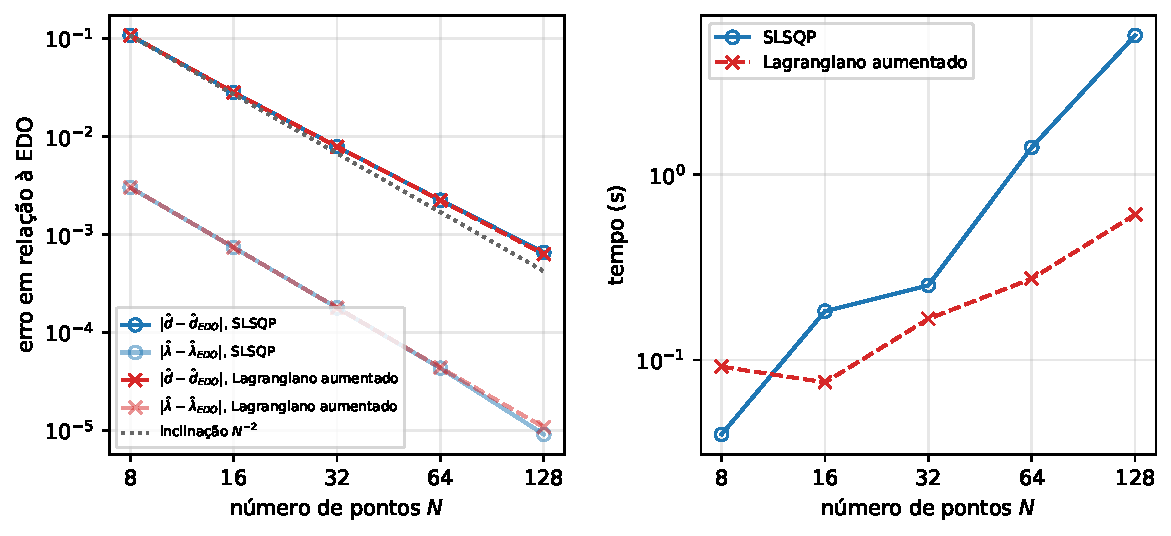
\includegraphics[width=\textwidth]{convergencia.pdf}
  \caption{Erro em relação à EDO (esquerda) e tempo de execução (direita) em função
    do número de pontos, para $\Vh = 2\Vh^*/3$ (Autoria própria)}
  \label{fig:convergencia}
\end{figure}

\subsection{Comportamento do lagrangiano aumentado}

A Figura~\ref{fig:historico} acompanha as iterações externas do lagrangiano aumentado
para $\Vh = \Vh^*/3$ e $N = 30$. No primeiro subproblema, com $\lambda_0 = 0$, a
violação é $|h| = \num{4.34e-3}$, praticamente igual à estimativa
$|\lambda^* - \lambda_0|/\mu_0 = \lh\,\Vh_0/\mu_0 = \num{4.33e-3}$ dada pela relação
$h \approx (\lambda^* - \lambda)/\mu$ da Seção~\ref{sec:la}. A partir daí, cada
atualização do multiplicador reduz a violação em duas a três ordens de grandeza, e o
critério $|h| \le 10^{-10}$ é atingido na quarta iteração, com $\mu = 8000$; o último
subproblema precisou de apenas duas iterações do L-BFGS-B. A medida de otimalidade, o
gradiente projetado do lagrangiano, fica em torno de $10^{-7}$ durante todo o processo,
o que mostra que cada subproblema foi resolvido com precisão. À direita, o
multiplicador converge para o do SLSQP a menos de \num{6e-8}, enquanto a diferença
para a EDO para em \num{1.3e-4}, que é o erro da discretização.

\begin{figure}[H]
  \centering
  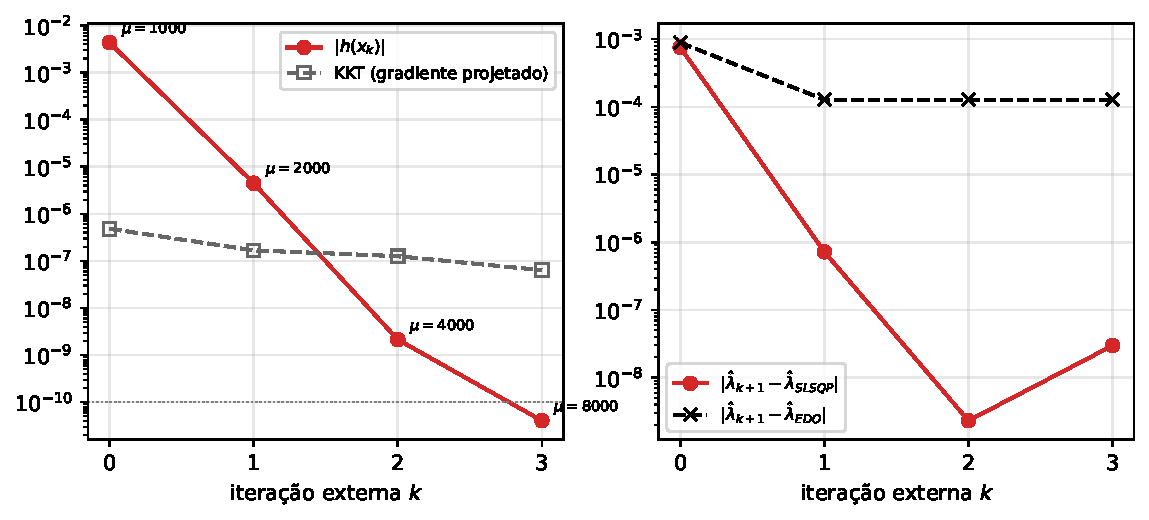
\includegraphics[width=\textwidth]{historico_al.pdf}
  \caption{Iterações externas do lagrangiano aumentado para $\Vh = \Vh^*/3$ e
    $N = 30$: violação da restrição e medida de otimalidade (esquerda) e erro do
    multiplicador (direita) (Autoria própria)}
  \label{fig:historico}
\end{figure}

\subsection{Multiplicador de Lagrange e pressão}

A Figura~\ref{fig:lambda-volume} compara, para 18 volumes, o multiplicador fornecido
pelo lagrangiano aumentado, com $N = 64$, com a pressão adimensional no plano do bico
calculada pela EDO, $(A - B\dhat)/\pi$. As duas curvas coincidem em toda a faixa, o que
confirma numericamente a Proposição~\ref{prop:multiplicador}: a diferença é menor que
\num{8.1e-5} até $\Vh = 30$ e cresce perto do volume máximo, chegando a \num{2.4e-3}
em $\Vh^*$. A pressão no bico cresce com o volume enquanto a gota é menor que uma
semiesfera, chega ao máximo perto de $\Vh = 2$ (a semiesfera, sem gravidade, teria
$\Vh = 2\pi/3 \approx \num{2.09}$) e depois diminui, porque o raio de curvatura volta
a crescer.

\begin{figure}[H]
  \centering
  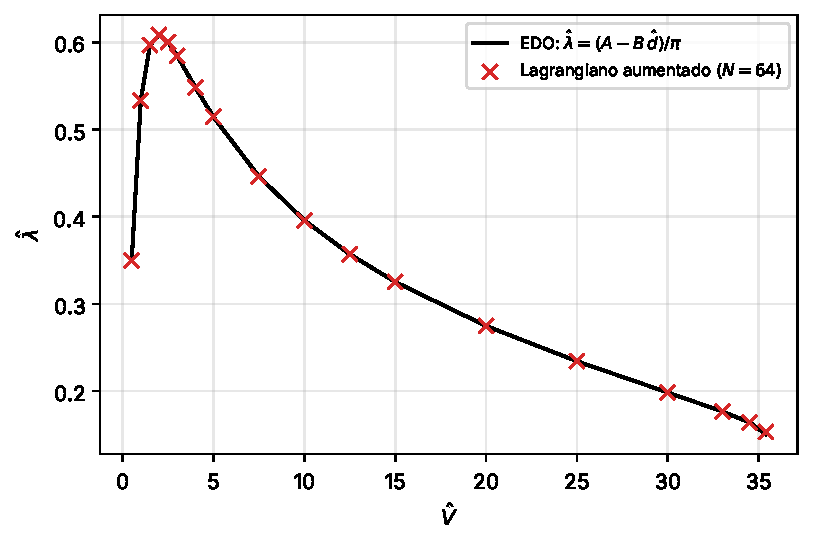
\includegraphics[width=0.8\textwidth]{lambda_volume.pdf}
  \caption{Multiplicador de Lagrange do lagrangiano aumentado e pressão adimensional no
    plano do bico obtida pela EDO, em função do volume (Autoria própria)}
  \label{fig:lambda-volume}
\end{figure}

\subsection{Gota tridimensional}

A Figura~\ref{fig:gota3d} e a Tabela~\ref{tab:gota3d} mostram a gota tridimensional de
volume $\Vh = 5$ pendurada no bico quadrado, com uma malha de 8 anéis e 16 setores
(145 vértices, dos quais 129 são variáveis, e 272 triângulos) e $B = \num{0.2695}$, o
mesmo usado em \code{src/3D/test.py}. Nos dois casos o SLSQP convergiu, em cerca de 200
iterações e de 25 a 32 segundos, com o volume correto até a precisão de máquina. Fixar
o anel do corte deixa a gota mais alta ($\dhat = \num{1.839}$ contra \num{1.632}) e
aumenta a energia em \qty{4.8}{\percent}, como se espera de um problema com mais
restrições.

\begin{figure}[H]
  \centering
  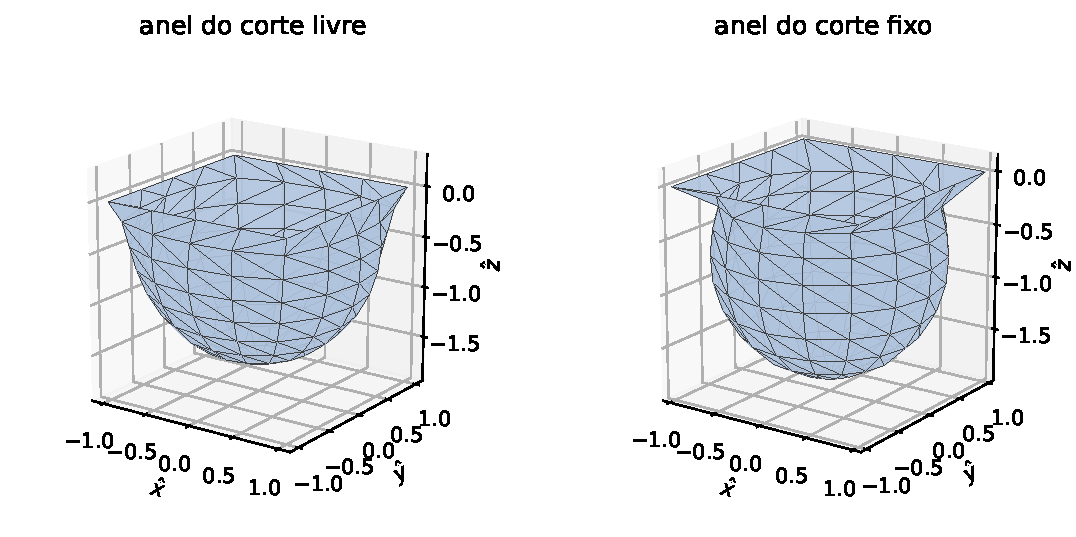
\includegraphics[width=\textwidth]{gota3d.pdf}
  \caption{Gota de volume $\Vh = 5$ pendurada em um bico quadrado, com o anel do corte
    da calota livre (esquerda) e fixo (direita) (Autoria própria)}
  \label{fig:gota3d}
\end{figure}

\begin{table}[H]
  \centering
  \caption{Resultados da gota tridimensional com bico quadrado e $\Vh = 5$ (Autoria própria)}
  \label{tab:gota3d}
  \begin{tabular}{lccccc}
\toprule
Anel do corte & Iterações & Tempo (s) & Volume obtido & Altura $\hat d$ & Energia $\hat E$ \\
\midrule
livre & 209 & \num{32.3} & \num{5.0000000000} & \num{1.6318} & \num{10.9628} \\
fixo & 200 & \num{24.6} & \num{5.0000000000} & \num{1.8386} & \num{11.4881} \\
\bottomrule
\end{tabular}

\end{table}

\section{Discussão}
\label{sec:discussao}

Os resultados confirmam que a forma de uma gota pendente pode ser obtida tanto pela
integração da equação de Young--Laplace quanto pela minimização da energia com
restrição de volume, e que o multiplicador de Lagrange dessa restrição é a pressão no
bico. Na formulação discreta, o SLSQP e o lagrangiano aumentado chegam à mesma
solução, e a diferença para a EDO, de segunda ordem em $N$, vem só da discretização do
perfil.

A vantagem de tempo do lagrangiano aumentado deve ser lida com cuidado. Ela vem
sobretudo do gradiente exato, que só escrevemos para o lagrangiano aumentado: o SLSQP
recebeu apenas a função objetivo e a restrição e estimou as derivadas por diferenças
finitas. Fornecer o mesmo gradiente ao SLSQP provavelmente reduziria bastante o seu
custo. Do ponto de vista do algoritmo, o que os resultados mostram é que o lagrangiano
aumentado resolve o problema com poucos subproblemas e com valores moderados de $\mu$,
sem o mal condicionamento da penalidade quadrática, como previsto pela relação
$h \approx (\lambda^* - \lambda)/\mu$.

Perto do volume máximo, a situação é mais delicada. O erro da discretização cresce
(\qty{2.2}{\percent} na altura com $N = 30$), porque a gota está no limite da
estabilidade e pequenas mudanças de forma quase não alteram a energia. Esse mesmo fato
tem uma consequência importante para o lagrangiano aumentado, ilustrada na
Figura~\ref{fig:descolamento}. Com $\mu_0 = 10$ em vez de $1000$, o primeiro
subproblema, que tem $\lambda = 0$, praticamente ignora a restrição e encolhe a gota. A
partir desse ponto, o método converge para outra solução do
Problema~\ref{prob:discreto}: 25 dos 29 pontos móveis colapsam no centro da calota,
sobre o limite $x_i = -1$, e o perfil passa pelo eixo, formando uma gota estrangulada,
já desprendida do bico. Essa configuração satisfaz a restrição de volume e tem energia
\qty{22}{\percent} menor ($\Eh = \num{30.64}$ contra \num{39.12}). Ou seja, a gota
pendente em $\Vh^*$ é apenas um mínimo local, e o método, partindo longe dela,
encontrou outro; fisicamente, trata-se do desprendimento da gota. Para evitar esse
comportamento, escolhemos $\mu_0$ grande o bastante para que o primeiro subproblema já
fique perto do volume desejado: pela relação acima, $|h| \approx \lh\,\Vh_0/\mu_0$,
que com $\mu_0 = 1000$ ficou abaixo de \qty{1}{\percent} em todos os casos testados. A
implementação também emite um aviso quando algum ponto chega ao limite $x_i = -1$.

\begin{figure}[H]
  \centering
  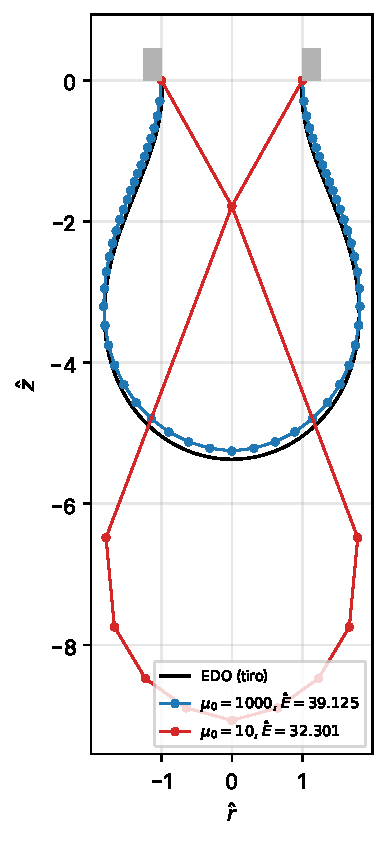
\includegraphics[width=0.45\textwidth]{descolamento.pdf}
  \caption{Gota de volume máximo obtida pelo lagrangiano aumentado com $\mu_0 = 1000$ e
    com $\mu_0 = 10$; no segundo caso o método converge para uma gota estrangulada, de
    energia menor (Autoria própria)}
  \label{fig:descolamento}
\end{figure}

Outro cuidado prático diz respeito ao critério de parada. O
Algoritmo~\ref{alg:lagrangiano-aumentado} aumenta $\mu$ a cada iteração. Quando a
tolerância pedida é menor que a precisão com que os subproblemas são resolvidos, por
exemplo com gradientes por diferenças finitas, a violação para de cair, $\mu$ continua
crescendo e a atualização $\lambda \leftarrow \lambda + \mu h$ passa a amplificar o
ruído de arredondamento de $h$. Em um dos nossos testes, com diferenças finitas e
tolerância $10^{-10}$, o multiplicador, que deveria valer $-0{,}5$, terminou em
$-7451$. Por isso a implementação interrompe o método quando um subproblema não altera
mais o ponto nem reduz a violação, informa que houve estagnação e mantém os
multiplicadores do último subproblema.

Na versão tridimensional, a formulação variacional funciona sem mudanças conceituais,
mas o custo é bem maior: com 129 variáveis e gradientes por diferenças finitas, o
SLSQP levou de 25 a 32 segundos. Além disso, a malha tem uma única camada de
triângulos entre o círculo da calota e o quadrado do bico, o que limita a precisão
perto da linha de contato, e não há uma solução de referência, como a EDO, para medir o
erro.

% ---------------------------------------------------------------------------
\chapter{Conclusão}

Neste trabalho, determinamos a forma de gotas pendentes de duas maneiras: integrando a
equação de Young--Laplace pelo método do tiro e minimizando a energia de superfície e
gravitacional com uma restrição de volume. A formulação variacional transforma um
problema clássico de capilaridade em um problema de otimização não linear com uma
restrição de igualdade, cujo multiplicador de Lagrange é a pressão no bico.

Implementamos o método do lagrangiano aumentado de \textcite{martins2021} com o SciPy,
usando o L-BFGS-B nos subproblemas, e o validamos reproduzindo o Exemplo 5.8 do livro.
Aplicado à gota, ele chegou à mesma solução discreta que o SLSQP e reproduziu a forma e
a pressão dadas pela EDO, com erro de segunda ordem no número de pontos. Com o
gradiente exato, precisou de 4 a 6 subproblemas e foi até sete vezes mais rápido que o
SLSQP com diferenças finitas. O estudo também mostrou dois cuidados práticos com o
método: o parâmetro de penalidade inicial deve ser grande o bastante para que o
primeiro subproblema não se afaste da restrição, sob pena de o método convergir para
outra solução, como a gota desprendida perto do volume máximo; e o critério de parada
deve ser compatível com a precisão dos subproblemas.

Por fim, a mesma formulação permitiu obter a forma de uma gota pendurada em um bico
quadrado, caso que a EDO axissimétrica não cobre. Os próximos passos são escrever o
gradiente exato na malha tridimensional, aplicar a ela o lagrangiano aumentado e
refinar a malha perto da linha de contato.

\printbibliography[heading=bibintoc, title={Referências}]

\end{document}
